\documentclass{standalone}
\usepackage{tikz}
\usetikzlibrary{patterns, positioning}
\usepackage[sfdefault]{ClearSans} %% option 'sfdefault' activates Clear Sans as the default text font
\usepackage[T1]{fontenc}

\begin{document}
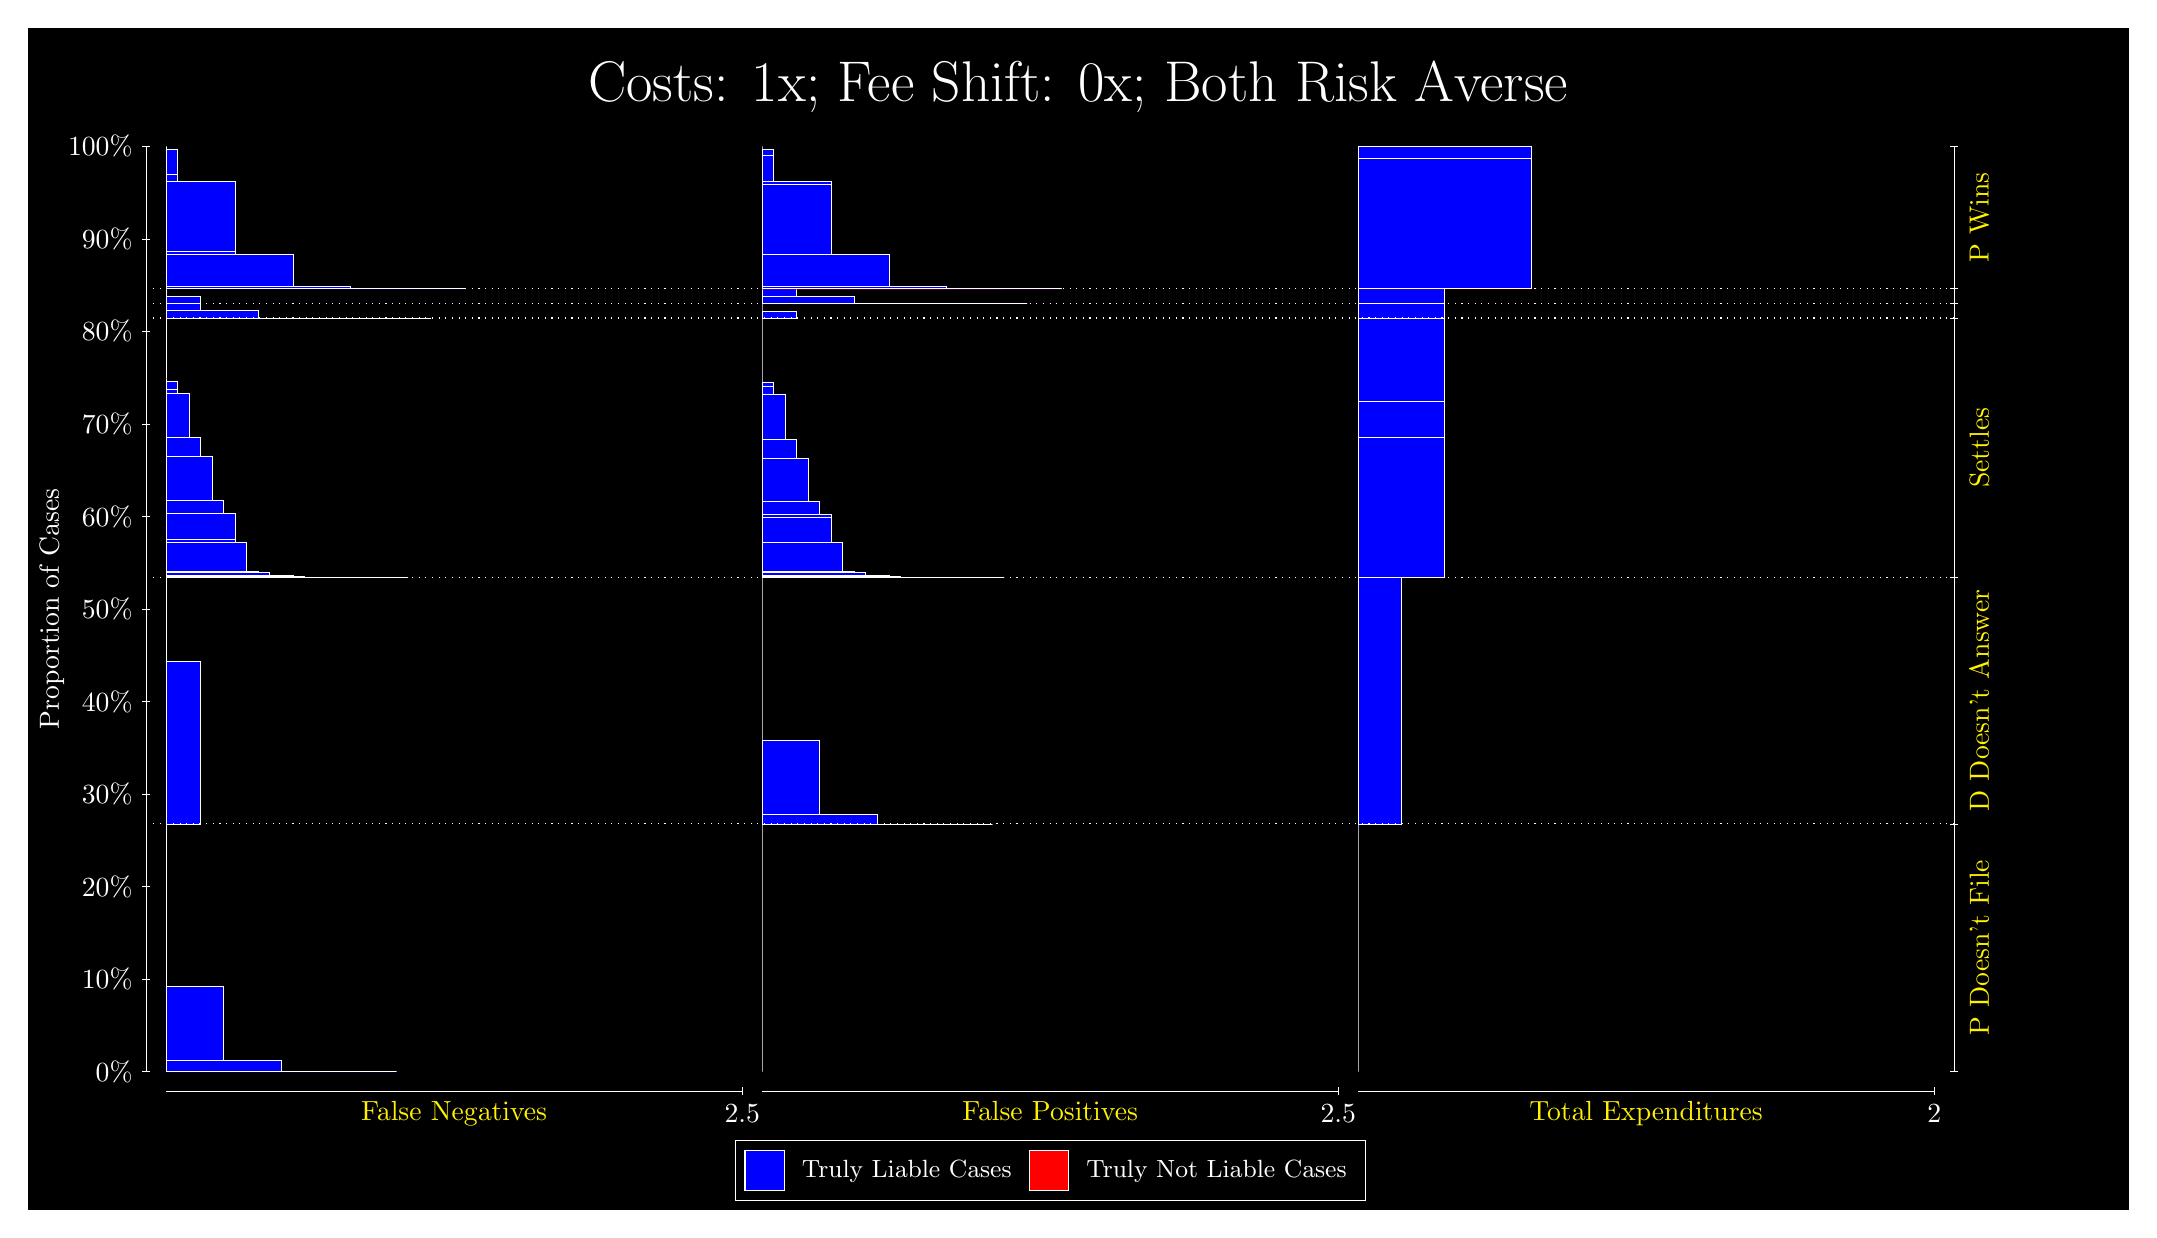
\begin{tikzpicture}
\draw[fill=black] (0,0) rectangle (26.667,15);
\draw[text=white] (0,13.5) rectangle (26.667,15) node[midway] {\huge Costs: 1x; Fee Shift: 0x; Both Risk Averse};
\draw[white, very thin] (1.5,1.75) -- (1.5,13.5);
\node[rotate=90, text=white, anchor=center] at (0.3, 7.625) {Proportion of Cases};
\draw[white, very thin] (1.45,1.75) -- (1.55,1.75);
\node[text=white, anchor=east] at (1.45, 1.75) {0\%};
\draw[white, very thin] (1.45,2.925) -- (1.55,2.925);
\node[text=white, anchor=east] at (1.45, 2.925) {10\%};
\draw[white, very thin] (1.45,4.1) -- (1.55,4.1);
\node[text=white, anchor=east] at (1.45, 4.1) {20\%};
\draw[white, very thin] (1.45,5.275) -- (1.55,5.275);
\node[text=white, anchor=east] at (1.45, 5.275) {30\%};
\draw[white, very thin] (1.45,6.45) -- (1.55,6.45);
\node[text=white, anchor=east] at (1.45, 6.45) {40\%};
\draw[white, very thin] (1.45,7.625) -- (1.55,7.625);
\node[text=white, anchor=east] at (1.45, 7.625) {50\%};
\draw[white, very thin] (1.45,8.8) -- (1.55,8.8);
\node[text=white, anchor=east] at (1.45, 8.8) {60\%};
\draw[white, very thin] (1.45,9.975) -- (1.55,9.975);
\node[text=white, anchor=east] at (1.45, 9.975) {70\%};
\draw[white, very thin] (1.45,11.15) -- (1.55,11.15);
\node[text=white, anchor=east] at (1.45, 11.15) {80\%};
\draw[white, very thin] (1.45,12.325) -- (1.55,12.325);
\node[text=white, anchor=east] at (1.45, 12.325) {90\%};
\draw[white, very thin] (1.45,13.5) -- (1.55,13.5);
\node[text=white, anchor=east] at (1.45, 13.5) {100\%};

\draw[white, very thin] (24.457,1.75) -- (24.457,13.5);
\draw[white, very thin] (24.407,1.75) -- (24.507,1.75);
\node[anchor=west] at (24.407, 1.75) {};
\draw[white, very thin] (24.407,4.8956) -- (24.507,4.8956);
\node[anchor=west] at (24.407, 4.8956) {};
\draw[white, very thin] (24.407,8.0263) -- (24.507,8.0263);
\node[anchor=west] at (24.407, 8.0263) {};
\draw[white, very thin] (24.407,11.32) -- (24.507,11.32);
\node[anchor=west] at (24.407, 11.32) {};
\draw[white, very thin] (24.407,11.505) -- (24.507,11.505);
\node[anchor=west] at (24.407, 11.505) {};
\draw[white, very thin] (24.407,11.691) -- (24.507,11.691);
\node[anchor=west] at (24.407, 11.691) {};
\draw[white, very thin] (24.407,13.5) -- (24.507,13.5);
\node[anchor=west] at (24.407, 13.5) {};

\draw[white, very thin, fill=blue] (1.75,1.75) rectangle (4.6775,1.75);
\draw[white, very thin, fill=blue] (1.75,1.75) rectangle (3.9457,1.7511);
\draw[white, very thin, fill=blue] (1.75,1.7511) rectangle (3.2138,1.8866);
\draw[white, very thin, fill=blue] (1.75,1.8866) rectangle (2.4819,2.8315);
\draw[white, very thin, fill=red] (1.75,2.8315) rectangle (1.75,2.8315);
\draw[white, very thin, fill=blue] (1.75,2.8315) rectangle (1.75,4.8956);
\draw[white, very thin, fill=blue] (1.75,4.8956) rectangle (2.1891,6.9603);
\draw[white, very thin, fill=red] (1.75,6.9603) rectangle (1.75,6.9603);
\draw[white, very thin, fill=blue] (1.75,6.9603) rectangle (1.75,8.0263);
\draw[white, very thin, fill=blue] (1.75,8.0263) rectangle (4.8239,8.0263);
\draw[white, very thin, fill=blue] (1.75,8.0263) rectangle (4.2384,8.0263);
\draw[white, very thin, fill=blue] (1.75,8.0263) rectangle (4.092,8.0263);
\draw[white, very thin, fill=blue] (1.75,8.0263) rectangle (3.9457,8.0263);
\draw[white, very thin, fill=blue] (1.75,8.0263) rectangle (3.6529,8.0264);
\draw[white, very thin, fill=blue] (1.75,8.0264) rectangle (3.5065,8.037);
\draw[white, very thin, fill=blue] (1.75,8.037) rectangle (3.3602,8.0564);
\draw[white, very thin, fill=blue] (1.75,8.0564) rectangle (3.2138,8.0568);
\draw[white, very thin, fill=blue] (1.75,8.0568) rectangle (3.0674,8.0868);
\draw[white, very thin, fill=blue] (1.75,8.0868) rectangle (2.921,8.1048);
\draw[white, very thin, fill=blue] (1.75,8.1048) rectangle (2.7746,8.4767);
\draw[white, very thin, fill=blue] (1.75,8.4767) rectangle (2.6283,8.5157);
\draw[white, very thin, fill=blue] (1.75,8.5157) rectangle (2.6283,8.8452);
\draw[white, very thin, fill=blue] (1.75,8.8452) rectangle (2.4819,8.9985);
\draw[white, very thin, fill=blue] (1.75,8.9985) rectangle (2.3355,9.562);
\draw[white, very thin, fill=blue] (1.75,9.562) rectangle (2.1891,9.8019);
\draw[white, very thin, fill=blue] (1.75,9.8019) rectangle (2.0428,10.36);
\draw[white, very thin, fill=blue] (1.75,10.36) rectangle (1.8964,10.409);
\draw[white, very thin, fill=blue] (1.75,10.409) rectangle (1.8964,10.515);
\draw[white, very thin, fill=blue] (1.75,10.515) rectangle (1.75,10.554);
\draw[white, very thin, fill=red] (1.75,10.554) rectangle (1.75,10.554);
\draw[white, very thin, fill=blue] (1.75,10.554) rectangle (1.75,11.32);
\draw[white, very thin, fill=blue] (1.75,11.32) rectangle (5.1167,11.32);
\draw[white, very thin, fill=blue] (1.75,11.32) rectangle (4.3848,11.32);
\draw[white, very thin, fill=blue] (1.75,11.32) rectangle (3.6529,11.322);
\draw[white, very thin, fill=blue] (1.75,11.322) rectangle (2.921,11.416);
\draw[white, very thin, fill=blue] (1.75,11.416) rectangle (2.1891,11.505);
\draw[white, very thin, fill=red] (1.75,11.505) rectangle (1.75,11.505);
\draw[white, very thin, fill=blue] (1.75,11.505) rectangle (2.1891,11.595);
\draw[white, very thin, fill=red] (1.75,11.595) rectangle (1.75,11.595);
\draw[white, very thin, fill=blue] (1.75,11.595) rectangle (1.75,11.691);
\draw[white, very thin, fill=blue] (1.75,11.691) rectangle (5.5558,11.691);
\draw[white, very thin, fill=blue] (1.75,11.691) rectangle (4.8239,11.691);
\draw[white, very thin, fill=blue] (1.75,11.691) rectangle (4.092,11.723);
\draw[white, very thin, fill=blue] (1.75,11.723) rectangle (3.3602,12.133);
\draw[white, very thin, fill=blue] (1.75,12.133) rectangle (2.6283,12.173);
\draw[white, very thin, fill=blue] (1.75,12.173) rectangle (2.6283,13.058);
\draw[white, very thin, fill=blue] (1.75,13.058) rectangle (1.8964,13.141);
\draw[white, very thin, fill=blue] (1.75,13.141) rectangle (1.8964,13.468);
\draw[white, very thin, fill=red] (1.75,13.468) rectangle (1.75,13.468);
\draw[white, very thin, fill=blue] (1.75,13.468) rectangle (1.75,13.5);
\draw[white, very thin, fill=red] (9.3189,1.75) rectangle (9.3189,1.75);
\draw[white, very thin, fill=blue] (9.3189,1.75) rectangle (9.3189,4.8956);
\draw[white, very thin, fill=red] (9.3189,4.8956) rectangle (12.246,4.8956);
\draw[white, very thin, fill=blue] (9.3189,4.8956) rectangle (12.246,4.8956);
\draw[white, very thin, fill=blue] (9.3189,4.8956) rectangle (11.515,4.8959);
\draw[white, very thin, fill=blue] (9.3189,4.8959) rectangle (10.783,5.0149);
\draw[white, very thin, fill=blue] (9.3189,5.0149) rectangle (10.051,5.9616);
\draw[white, very thin, fill=blue] (9.3189,5.9616) rectangle (9.3189,8.0263);
\draw[white, very thin, fill=red] (9.3189,8.0263) rectangle (12.393,8.0263);
\draw[white, very thin, fill=blue] (9.3189,8.0263) rectangle (12.393,8.0263);
\draw[white, very thin, fill=red] (9.3189,8.0263) rectangle (11.807,8.0263);
\draw[white, very thin, fill=blue] (9.3189,8.0263) rectangle (11.807,8.0263);
\draw[white, very thin, fill=blue] (9.3189,8.0263) rectangle (11.661,8.0263);
\draw[white, very thin, fill=red] (9.3189,8.0263) rectangle (11.515,8.0263);
\draw[white, very thin, fill=blue] (9.3189,8.0263) rectangle (11.515,8.0263);
\draw[white, very thin, fill=red] (9.3189,8.0263) rectangle (11.222,8.0263);
\draw[white, very thin, fill=blue] (9.3189,8.0263) rectangle (11.222,8.0264);
\draw[white, very thin, fill=blue] (9.3189,8.0264) rectangle (11.075,8.0369);
\draw[white, very thin, fill=blue] (9.3189,8.0369) rectangle (10.929,8.0557);
\draw[white, very thin, fill=red] (9.3189,8.0557) rectangle (10.929,8.0557);
\draw[white, very thin, fill=blue] (9.3189,8.0557) rectangle (10.929,8.0558);
\draw[white, very thin, fill=blue] (9.3189,8.0558) rectangle (10.783,8.0562);
\draw[white, very thin, fill=red] (9.3189,8.0562) rectangle (10.636,8.0562);
\draw[white, very thin, fill=blue] (9.3189,8.0562) rectangle (10.636,8.0859);
\draw[white, very thin, fill=blue] (9.3189,8.0859) rectangle (10.49,8.1);
\draw[white, very thin, fill=blue] (9.3189,8.1) rectangle (10.344,8.471);
\draw[white, very thin, fill=blue] (9.3189,8.471) rectangle (10.197,8.7926);
\draw[white, very thin, fill=blue] (9.3189,8.7926) rectangle (10.197,8.8314);
\draw[white, very thin, fill=red] (9.3189,8.8314) rectangle (10.051,8.8314);
\draw[white, very thin, fill=blue] (9.3189,8.8314) rectangle (10.051,8.9859);
\draw[white, very thin, fill=blue] (9.3189,8.9859) rectangle (9.9044,9.5444);
\draw[white, very thin, fill=blue] (9.3189,9.5444) rectangle (9.758,9.7844);
\draw[white, very thin, fill=blue] (9.3189,9.7844) rectangle (9.6116,10.348);
\draw[white, very thin, fill=blue] (9.3189,10.348) rectangle (9.4652,10.453);
\draw[white, very thin, fill=blue] (9.3189,10.453) rectangle (9.4652,10.501);
\draw[white, very thin, fill=blue] (9.3189,10.501) rectangle (9.3189,11.32);
\draw[white, very thin, fill=red] (9.3189,11.32) rectangle (9.758,11.32);
\draw[white, very thin, fill=blue] (9.3189,11.32) rectangle (9.758,11.41);
\draw[white, very thin, fill=blue] (9.3189,11.41) rectangle (9.3189,11.505);
\draw[white, very thin, fill=red] (9.3189,11.505) rectangle (12.686,11.505);
\draw[white, very thin, fill=blue] (9.3189,11.505) rectangle (12.686,11.505);
\draw[white, very thin, fill=blue] (9.3189,11.505) rectangle (11.954,11.505);
\draw[white, very thin, fill=blue] (9.3189,11.505) rectangle (11.222,11.507);
\draw[white, very thin, fill=blue] (9.3189,11.507) rectangle (10.49,11.601);
\draw[white, very thin, fill=blue] (9.3189,11.601) rectangle (9.758,11.691);
\draw[white, very thin, fill=red] (9.3189,11.691) rectangle (13.125,11.691);
\draw[white, very thin, fill=blue] (9.3189,11.691) rectangle (13.125,11.691);
\draw[white, very thin, fill=red] (9.3189,11.691) rectangle (12.393,11.691);
\draw[white, very thin, fill=blue] (9.3189,11.691) rectangle (12.393,11.691);
\draw[white, very thin, fill=red] (9.3189,11.691) rectangle (11.661,11.691);
\draw[white, very thin, fill=blue] (9.3189,11.691) rectangle (11.661,11.723);
\draw[white, very thin, fill=red] (9.3189,11.723) rectangle (10.929,11.723);
\draw[white, very thin, fill=blue] (9.3189,11.723) rectangle (10.929,12.133);
\draw[white, very thin, fill=blue] (9.3189,12.133) rectangle (10.197,13.018);
\draw[white, very thin, fill=red] (9.3189,13.018) rectangle (10.197,13.018);
\draw[white, very thin, fill=blue] (9.3189,13.018) rectangle (10.197,13.058);
\draw[white, very thin, fill=blue] (9.3189,13.058) rectangle (9.4652,13.384);
\draw[white, very thin, fill=blue] (9.3189,13.384) rectangle (9.4652,13.468);
\draw[white, very thin, fill=blue] (9.3189,13.468) rectangle (9.3189,13.5);
\draw[white, very thin, fill=red] (16.888,1.75) rectangle (16.888,1.75);
\draw[white, very thin, fill=blue] (16.888,1.75) rectangle (16.888,4.8956);
\draw[white, very thin, fill=red] (16.888,4.8956) rectangle (17.437,4.8956);
\draw[white, very thin, fill=blue] (16.888,4.8956) rectangle (17.437,8.0263);
\draw[white, very thin, fill=red] (16.888,8.0263) rectangle (17.986,8.0263);
\draw[white, very thin, fill=blue] (16.888,8.0263) rectangle (17.986,9.8069);
\draw[white, very thin, fill=red] (16.888,9.8069) rectangle (17.986,9.8069);
\draw[white, very thin, fill=blue] (16.888,9.8069) rectangle (17.986,10.262);
\draw[white, very thin, fill=red] (16.888,10.262) rectangle (17.986,10.262);
\draw[white, very thin, fill=blue] (16.888,10.262) rectangle (17.986,11.32);
\draw[white, very thin, fill=red] (16.888,11.32) rectangle (17.986,11.32);
\draw[white, very thin, fill=blue] (16.888,11.32) rectangle (17.986,11.505);
\draw[white, very thin, fill=red] (16.888,11.505) rectangle (17.986,11.505);
\draw[white, very thin, fill=blue] (16.888,11.505) rectangle (17.986,11.691);
\draw[white, very thin, fill=red] (16.888,11.691) rectangle (19.083,11.691);
\draw[white, very thin, fill=blue] (16.888,11.691) rectangle (19.083,13.354);
\draw[white, very thin, fill=red] (16.888,13.354) rectangle (19.083,13.354);
\draw[white, very thin, fill=blue] (16.888,13.354) rectangle (19.083,13.5);
\draw[white, dotted] (1.5,4.8956) -- (24.457,4.8956);
\draw[white, dotted] (1.5,8.0263) -- (24.457,8.0263);
\draw[white, dotted] (1.5,11.32) -- (24.457,11.32);
\draw[white, dotted] (1.5,11.505) -- (24.457,11.505);
\draw[white, dotted] (1.5,11.691) -- (24.457,11.691);
\draw[white, very thin] (1.75,1.5) -- (9.0689,1.5);
\node[text=yellow, anchor=north] at (5.4094, 1.5) {False Negatives};
\draw[white, very thin] (9.0689,1.45) -- (9.0689,1.55);
\node[text=white, anchor=north] at (9.0689, 1.45) {2.5};

\draw[white, very thin] (9.3189,1.5) -- (16.638,1.5);
\node[text=yellow, anchor=north] at (12.978, 1.5) {False Positives};
\draw[white, very thin] (16.638,1.45) -- (16.638,1.55);
\node[text=white, anchor=north] at (16.638, 1.45) {2.5};

\draw[white, very thin] (16.888,1.5) -- (24.207,1.5);
\node[text=yellow, anchor=north] at (20.547, 1.5) {Total Expenditures};
\draw[white, very thin] (24.207,1.45) -- (24.207,1.55);
\node[text=white, anchor=north] at (24.207, 1.45) {2};

\node[text=yellow, centered, rotate=90] at (24.777, 3.3228) {P Doesn't File};
\node[text=yellow, centered, rotate=90] at (24.777, 6.4609) {D Doesn't Answer};
\node[text=yellow, centered, rotate=90] at (24.777, 9.6732) {Settles};


\node[text=yellow, centered, rotate=90] at (24.777, 12.595) {P Wins};

\draw (12.978300999999998,1.5) node[draw=none] (baseCoordinate) {};
\begin{scope}[align=center]
        \matrix[scale=0.5, draw=white, below=0.5cm of baseCoordinate, nodes={draw}, column sep=0.1cm]{
            \node[rectangle, draw, minimum width=0.5cm, minimum height=0.5cm, fill=blue] {}; &
            \node[draw=none, font=\small, text=white] (B) {Truly Liable Cases}; &
            \node[rectangle, draw, minimum width=0.5cm, minimum height=0.5cm, fill=red] {}; &
            \node[draw=none, font=\small, text=white] (B) {Truly Not Liable Cases}; \\
            };
\end{scope}

\end{tikzpicture}
\end{document}